\subsection{Simulation results: binary-continuous mix}

We start by considering a mix of binary and continuous variables generated as outlined in Section \ref{sec::setup} to be able to compare results with those of \citet{Fan17}. For this purpose, \figref{fig:bench_binary} depicts the mean estimation error $\Norm{\hat{\boldsymbol\Omega} - \boldsymbol\Omega^*}_F$ and the AUC for the different estimators under the different $(d,n)$ regimes.
%Table \ref{kendall_table} reports mean estimation errors $\Norm{\hat{\boldsymbol\Omega} - \boldsymbol\Omega^*}_F$ under the different $(d,n)$ regimes. When for all $j$, $f_j(x) = x$ we recover the latent Gaussian and when $f_j(x) = x^3$ the latent Gaussian copula model.

The oracle estimator in the third column of Table \ref{kendall_table} corresponds to estimating $\hat{\boldsymbol\Sigma}^{(n)}$ from Definition \ref{def1} based on realization of the latent data $(\boldsymbol{Z_1},\boldsymbol{Z_2})$. Next in column four, the binary $\hat{\boldsymbol\Omega}_\tau$ indicates the nonparanormal estimator proposed by \citet{Fan17}. The next two columns, namely $\hat{\boldsymbol\Omega}_{\text{MLE}}$ and $\hat{\boldsymbol\Omega}_r$ indicate the ML approach and the general mixed estimator developed in Sections \ref{sec::latent_gaussian} and \ref{sec::nonparanormal}, respectively.
%
%\begin{table}[htbp!] 
    %\centering 
    %\begin{longtable}{\textwidth}{c @{\extracolsep{\fill}} clcccc}
    \begin{longtable}[c]{@{}*{6}{>{\arraybackslash}p{0.135\linewidth}}@{}}
    \caption{Binary mixed data structure learning; Simulated data with $100$ simulation runs. Standard errors in brackets\label{kendall_table}}
    \\[-1.8ex]\hline 
    \hline \\[-1.8ex] 
    $d,n,f(x)$ && Oracle $\hat{\boldsymbol\Omega}$ & binary $\hat{\boldsymbol\Omega}_{\tau}$ & $\hat{\boldsymbol\Omega}_{\text{MLE}}$ & $\hat{\boldsymbol\Omega}_r$ \\ 
    \hline \\[-1.8ex] 
    \endfirsthead
    \endhead
    
    \multirow{8}{*}{$50,200,x$} & $\Norm{\hat{\Omega} - \Omega}_F$ & $2.858$ & $3.126$ & $3.095$ & $3.111$ \\ [-.25em]
    &  & \footnotesize{($0.096$)} & \footnotesize{($0.172$)} & \footnotesize{($0.143$)} & \footnotesize{($0.151$)} \\  [.15em] 
    &FPR & $0.016$ & $0.250$ & $0.222$ & $0.231$ \\ [-.25em]
    & & \footnotesize{($0.005$)} & \footnotesize{($0.104$)} & \footnotesize{($0.092$)} & \footnotesize{($0.102$)} \\ [.15em]
    &TPR & $0.340$ & $0.587$ & $0.566$ & $0.567$ \\   [-.25em]
    & & \footnotesize{($0.042$)} & \footnotesize{($0.108$)} & \footnotesize{($0.111$)} & \footnotesize{($0.118$)} \\  [.15em]
    &AUC & $0.880$ & $0.713$ & $0.720$ & $0.715$ \\  [-.25em]
    & & \footnotesize{($0.014$)} & \footnotesize{($0.020$)} & \footnotesize{($0.020$)} & \footnotesize{($0.020$)} \\  [1em]
    
    %
    \multirow{8}{*}{$50,200,x^3$} & $\Norm{\hat{\Omega} - \Omega}_F$ & $2.851$ & $3.153$ & $3.241$ & $3.115$ \\  [-.25em]
    & & \footnotesize{($0.115$)} & \footnotesize{($0.167$)} & \footnotesize{($0.115$)} & \footnotesize{($0.147$)} \\ [.15em]
    & FPR & $0.016$ & $0.263$ & $0.187$ & $0.228$ \\  [-.25em]
    & & \footnotesize{($0.006$)} & \footnotesize{($0.111$)} & \footnotesize{($0.059$)} & \footnotesize{($0.097$)} \\ [.15em]
    & TPR & $0.345$ & $0.604$ & $0.410$ & $0.576$ \\ [-.25em]
    & & \footnotesize{($0.052$)} & \footnotesize{($0.125$)} & \footnotesize{($0.090$)} & \footnotesize{($0.120$)} \\ [.15em]
    & AUC & $0.881$ & $0.718$ & $0.650$ & $0.721$ \\ [-.25em]
    & & \footnotesize{($0.014$)} & \footnotesize{($0.021$)} & \footnotesize{($0.021$)} & \footnotesize{($0.022$)} \\   [1em]
    %
    %
    \multirow{8}{*}{$250,200,x$} & $\Norm{\hat{\Omega} - \Omega}_F$ & $3.186$ & $4.090$ & $4.099$ & $4.098$ \\  [-.25em]
    & & \footnotesize{($0.103$)} & \footnotesize{($0.115$)} & \footnotesize{($0.108$)} & \footnotesize{($0.115$)} \\ [.15em] 
    & FPR & $0.006$ & $0.040$ & $0.039$ & $0.039$ \\ [-.25em]
    & & \footnotesize{($0.001$)} & \footnotesize{($0.005$)} & \footnotesize{($0.004$)} & \footnotesize{($0.004$)} \\ [.15em]
    & TPR & $0.304$ & $0.222$ & $0.228$ & $0.224$ \\ [-.25em]
    & & \footnotesize{($0.037$)} & \footnotesize{($0.034$)} & \footnotesize{($0.033$)} & \footnotesize{($0.034$)} \\ [.15em]
    & AUC & $0.884$ & $0.717$ & $0.726$ & $0.720$ \\ [-.25em]
    & & \footnotesize{($0.015$)} & \footnotesize{($0.018$)} & \footnotesize{($0.018$)} & \footnotesize{($0.018$)} \\  [1em]
    %
    %
    \multirow{8}{*}{$250,200,x^3$} & $\Norm{\hat{\Omega} - \Omega}_F$ & $3.194$ & $4.086$ & $4.287$ & $4.105$ \\  [-.25em]
    & & \footnotesize{($0.098$)} & \footnotesize{($0.098$)} & \footnotesize{($0.112$)} & \footnotesize{($0.109$)} \\ [.15em]
    & FPR & $0.006$ & $0.040$ & $0.042$ & $0.040$ \\  [-.25em]
    & & \footnotesize{($0.001$)} & \footnotesize{($0.004$)} & \footnotesize{($0.004$)} & \footnotesize{($0.005$)} \\ [.15em]
    & TPR & $0.304$ & $0.223$ & $0.144$ & $0.226$ \\ [-.25em]
    & & \footnotesize{($0.039$)} & \footnotesize{($0.033$)} & \footnotesize{($0.025$)} & \footnotesize{($0.031$)} \\  [.15em] 
    & AUC & $0.883$ & $0.716$ & $0.649$ & $0.719$ \\  [-.25em]
    & & \footnotesize{($0.012$)} & \footnotesize{($0.017$)} & \footnotesize{($0.018$)} & \footnotesize{($0.017$)} \\  [1em]
    %
    %
    \multirow{8}{*}{$750,300,x$} & $\Norm{\hat{\Omega} - \Omega}_F$ & $11.187$ & $10.264$ & $10.265$ & $10.270$ \\  [-.25em] 
    & & \footnotesize{($0.134$)} & \footnotesize{($0.129$)} & \footnotesize{($0.137$)} & \footnotesize{($0.128$)} \\ [.15em]
    & FPR & $0.256$ & $0.142$ & $0.144$ & $0.143$ \\ [-.25em]
    & & \footnotesize{($0.007$)} & \footnotesize{($0.005$)} & \footnotesize{($0.006$)} & \footnotesize{($0.005$)} \\ [.15em] 
    & TPR & $0.938$ & $0.602$ & $0.619$ & $0.611$ \\ [-.25em]
    & & \footnotesize{($0.009$)} & \footnotesize{($0.021$)} & \footnotesize{($0.022$)} & \footnotesize{($0.022$)} \\ [.15em]
    & AUC & $0.939$ & $0.770$ & $0.777$ & $0.774$ \\ [-.25em]
    & & \footnotesize{($0.006$)} & \footnotesize{($0.010$)} & \footnotesize{($0.010$)} & \footnotesize{($0.010$)} \\ [1em]
    %
    %
    \multirow{8}{*}{$750,300,x^3$} & $\Norm{\hat{\Omega} - \Omega}_F$ & $11.197$ & $10.273$ & $10.845$ & $10.287$ \\ [-.25em]
    & & \footnotesize{($0.138$)} & \footnotesize{($0.127$)} & \footnotesize{($0.115$)} & \footnotesize{($0.121$)} \\ [.15em] 
    & FPR & $0.256$ & $0.142$ & $0.136$ & $0.144$ \\ [-.25em]
    & & \footnotesize{($0.007$)} & \footnotesize{($0.005$)} & \footnotesize{($0.004$)} & \footnotesize{($0.005$)} \\ [.15em]
    & TPR & $0.937$ & $0.601$ & $0.455$ & $0.611$ \\ [-.25em]
    & & \footnotesize{($0.008$)} & \footnotesize{($0.018$)} & \footnotesize{($0.020$)} & \footnotesize{($0.019$)} \\ [.15em]
    & AUC & $0.938$ & $0.769$ & $0.695$ & $0.773$ \\ [-.25em]
    & & \footnotesize{($0.005$)} & \footnotesize{($0.009$)} & \footnotesize{($0.010$)} & \footnotesize{($0.009$)} \\ 
    \hline \\[-1.8ex] 
    \end{longtable}
%\end{table}



\begin{figure}
    \centering
    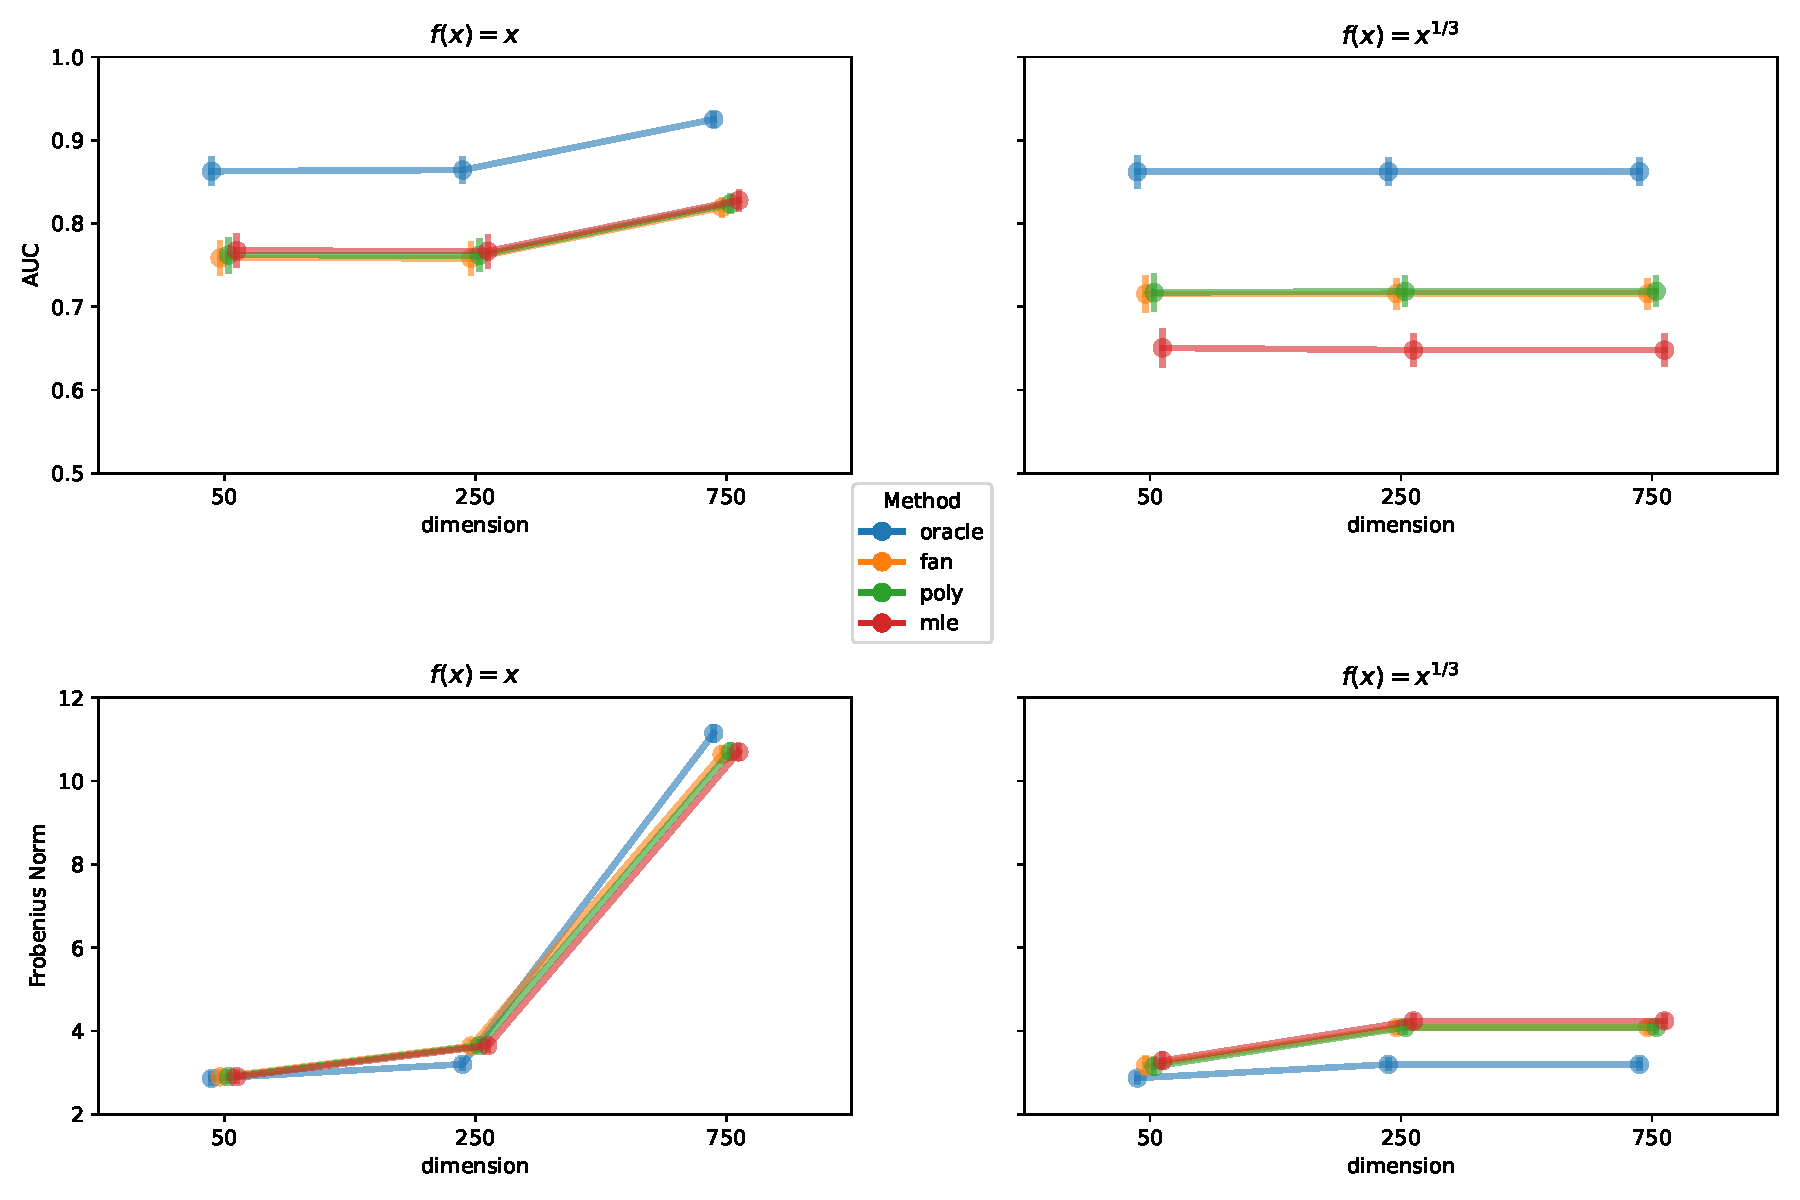
\includegraphics[width=\textwidth]{Figures/binary.pdf}
    \caption{Binary benchmark results}
    \label{fig:bench_binary}
\end{figure}

As expected, the estimation error for $d = 50$ and $n=200$ in the latent Gaussian setting is almost identical for $\hat{\boldsymbol\Omega}_\tau$ and our proposed nonparanormal estimator $\hat{\boldsymbol\Omega}_r$. Additionally, $\hat{\boldsymbol\Omega}_{\text{MLE}}$ performs best in this case. Compared to the oracle estimator, all three approaches exhibit very little loss in accuracy that arises due to binarization. Looking at graph recovery in terms of FPR, TPR, and AUC the picture is similar.
%For $\hat{\boldsymbol\Omega}_\tau$, $\hat{\boldsymbol\Omega}_{\text{MLE}}$, and $\hat{\boldsymbol\Omega}_r$ the FPR is around $22-25\%$ while the TPR amounts to $56-58\%$. Together, they form the AUC amounting to around $0.71$. Note, that the oracle estimator produces fewer TPs at a much lower FPR. The reason for the relatively low TPR is the fact that the glasso penalty induces too much sparsity in this low-dimensional setting. On the other hand, $\hat{\boldsymbol\Omega}_\tau$, $\hat{\boldsymbol\Omega}_{\text{MLE}}$, and $\hat{\boldsymbol\Omega}_r$ seem to be less conservative and produce more FPs.

Turning to the nonparanormal setting with $f_j(x) = x^3$ under $d = 50$ and $n=200$, as expected $\hat{\boldsymbol\Omega}_\tau$ and $\hat{\boldsymbol\Omega}_r$ remain largely unchanged but for small numerical differences. However, for $\hat{\boldsymbol\Omega}_{\text{MLE}}$ accuracy, both in terms of estimation error and graph recovery drops noticeably. However, the FPR remains unchanged, indicating that whilst detecting fewer correct edges in the graph the number of incorrect edges is not affected by this particular transformation. When increasing the number of variables to $d=250$ and $d=750$ the picture is similar to before. To sum up, when compared to the estimator $\hat{\boldsymbol\Omega}_\tau$ proposed by \citet{Fan17} both $\hat{\boldsymbol\Omega}_{\text{MLE}}$ and $\hat{\boldsymbol\Omega}_r$ perform similarly, under the latent Gaussian assumption even somewhat better. $\hat{\boldsymbol\Omega}_r$ performs slightly better than $\hat{\boldsymbol\Omega}_\tau$ in all scenarios considered. The loss of accuracy that arises from the discretization is not too severe under all $(d,n)$ regimes considered. Note, that the binary-continuous mix is merely a special case of the general mixed data scheme we consider in our paper. Therefore, being able to show similar or even improved performance to the current gold standard is important.

\subsection{Arbitrary mixed data results}

We turn to the set of experiments where we generate a mix of continuous and discrete data with arbitrary numbers of levels. As existing approaches, and in particular the bridge function approach, do not extend to this fully general case, we can no longer compare the proposed method to an existing one. Instead in Table \ref{mix_table}, we report a second oracle estimator, namely oracle $\hat{\Omega}_\rho$, i.e. applying Definition \ref{case1_nonpara} to realization from $\boldsymbol{Z} = (\boldsymbol{Z}_1, \boldsymbol{X}_2)$ in order to get more insight into the cases where $f_j(x) = x^3$.

When comparing $\Norm{\hat{\boldsymbol\Omega} - \boldsymbol\Omega^*}_F$ across the different settings, similar to the previous results, efficiency loss is almost negligible.

%\begin{table}[htbp!] 
    %\centering 
    
    %\begin{tabular*}{\textwidth}{c @{\extracolsep{\fill}} clcccc}
    \begin{longtable}[c]{@{}*{6}{>{\arraybackslash}p{0.135\linewidth}}@{}}
    \caption{General mixed data structure learning; Simulated data with $100$ simulation runs. Standard errors in brackets \label{mix_table}}
    \\[-1.8ex]\hline 
    \hline \\[-1.8ex] 
    $d,n,f(x)$ && Oracle $\hat{\Omega}$ & Oracle $\hat{\Omega}_{\rho}$ & $\hat{\Omega}_{\text{MLE}}$ & $\hat{\Omega}_r$ \\ 
    \hline \\[-1.8ex] 
    \multirow{8}{*}{$50,200,x$} & $\Norm{\hat{\Omega} - \Omega}_F$ & $2.860$ & $2.845$ & $2.892$ & $2.890$ \\ [-.25em]
    & & \footnotesize{($0.091$)} & \footnotesize{($0.097$)} & \footnotesize{($0.096$)} & \footnotesize{($0.097$)} \\ [.15em]
    & FPR & $0.015$ & $0.019$ & $0.042$ & $0.044$ \\ [-.25em]
    & & \footnotesize{($0.005$)} & \footnotesize{($0.005$)} & \footnotesize{($0.012$)} & \footnotesize{($0.012$)} \\ [.15em]
    & TPR & $0.335$ & $0.343$ & $0.356$ & $0.356$ \\ [-.25em]
    & & \footnotesize{($0.043$)} & \footnotesize{($0.044$)} & \footnotesize{($0.061$)} & \footnotesize{($0.059$)} \\ [.15em]
    & AUC & $0.881$ & $0.864$ & $0.816$ & $0.811$ \\ [-.25em]
    & & \footnotesize{($0.013$)} & \footnotesize{($0.015$)} & \footnotesize{($0.018$)} & \footnotesize{($0.017$)} \\  [1em]
    %
    %
    \multirow{8}{*}{$50,200,x^3$} & $\Norm{\hat{\Omega} - \Omega}_F$ & $2.869$ & $2.866$ & $3.014$ & $2.912$ \\ [-.25em]
    & & \footnotesize{($0.101$)} & \footnotesize{($0.104$)} & \footnotesize{($0.094$)} & \footnotesize{($0.099$)} \\ [.15em] 
    & FPR & $0.016$ & $0.019$ & $0.044$ & $0.042$ \\ [-.25em]
    & & \footnotesize{($0.005$)} & \footnotesize{($0.007$)} & \footnotesize{($0.011$)} & \footnotesize{($0.010$)} \\ [.15em]
    & TPR & $0.336$ & $0.338$ & $0.244$ & $0.352$ \\ [-.25em]
    & & \footnotesize{($0.047$)} & \footnotesize{($0.049$)} & \footnotesize{($0.041$)} & \footnotesize{($0.053$)} \\ [.15em]
    & AUC & $0.879$ & $0.862$ & $0.730$ & $0.807$ \\ [-.25em]
    & & \footnotesize{($0.015$)} & \footnotesize{($0.015$)} & \footnotesize{($0.021$)} & \footnotesize{($0.018$)} \\ [1em]
    %
    %
    \multirow{8}{*}{$250,200,x$} & $\Norm{\hat{\Omega} - \Omega}_F$ & $3.201$ & $3.212$ & $3.503$ & $3.507$ \\ [-.25em]
    & & \footnotesize{($0.109$)} & \footnotesize{($0.108$)} & \footnotesize{($0.104$)} & \footnotesize{($0.104$)} \\ [.15em]
    & FPR & $0.006$ & $0.008$ & $0.016$ & $0.016$ \\ [-.25em]
    & & \footnotesize{($0.001$)} & \footnotesize{($0.002$)} & \footnotesize{($0.002$)} & \footnotesize{($0.002$)} \\ [.15em]
    & TPR & $0.297$ & $0.300$ & $0.257$ & $0.255$ \\ [-.25em]
    & & \footnotesize{($0.040$)} & \footnotesize{($0.037$)} & \footnotesize{($0.038$)} & \footnotesize{($0.037$)} \\ [.15em]
    & AUC & $0.879$ & $0.861$ & $0.816$ & $0.811$ \\ [-.25em]
    & & \footnotesize{($0.015$)} & \footnotesize{($0.015$)} & \footnotesize{($0.016$)} & \footnotesize{($0.017$)} \\  [1em]
    %
    %
    \multirow{8}{*}{$250,200,x^3$} & $\Norm{\hat{\Omega} - \Omega}_F$ & $3.192$ & $3.209$ & $3.708$ & $3.503$ \\ [-.25em]
    & & \footnotesize{($0.092$)} & \footnotesize{($0.091$)} & \footnotesize{($0.096$)} & \footnotesize{($0.090$)} \\ [.15em]
    & FPR & $0.006$ & $0.008$ & $0.018$ & $0.017$ \\ [-.25em]
    & & \footnotesize{($0.001$)} & \footnotesize{($0.001$)} & \footnotesize{($0.002$)} & \footnotesize{($0.002$)} \\ [.15em]
    & TPR & $0.300$ & $0.289$ & $0.153$ & $0.255$ \\ [-.25em]
    & & \footnotesize{($0.036$)} & \footnotesize{($0.033$)} & \footnotesize{($0.022$)} & \footnotesize{($0.037$)} \\ [.15em]
    & AUC & $0.881$ & $0.863$ & $0.734$ & $0.812$ \\ [-.25em]
    & & \footnotesize{($0.012$)} & \footnotesize{($0.013$)} & \footnotesize{($0.017$)} & \footnotesize{($0.015$)} \\  [1em]
    %
    %
    \multirow{8}{*}{$750,300,x$} & $\Norm{\hat{\Omega} - \Omega}_F$ & $11.207$ & $11.154$ & $10.913$ & $10.928$ \\ [-.25em]
    & & \footnotesize{($0.140$)} & \footnotesize{($0.148$)} & \footnotesize{($0.125$)} & \footnotesize{($0.128$)} \\ [.15em] 
    & FPR & $0.257$ & $0.247$ & $0.214$ & $0.213$ \\ [-.25em]
    & & \footnotesize{($0.007$)} & \footnotesize{($0.007$)} & \footnotesize{($0.007$)} & \footnotesize{($0.007$)} \\ [.15em]
    & TPR & $0.936$ & $0.917$ & $0.835$ & $0.830$ \\ [-.25em]
    & & \footnotesize{($0.010$)} & \footnotesize{($0.011$)} & \footnotesize{($0.016$)} & \footnotesize{($0.014$)} \\ [.15em]
    & AUC & $0.938$ & $0.925$ & $0.878$ & $0.874$ \\ [-.25em]
    & & \footnotesize{($0.006$)} & \footnotesize{($0.006$)} & \footnotesize{($0.008$)} & \footnotesize{($0.008$)} \\  [1em]
    %
    \multirow{8}{*}{$750,300,x^3$} & $\Norm{\hat{\Omega} - \Omega}_F$ & $11.199$ & $11.165$ & $11.398$ & $10.939$ \\ [-.25em] 
    & & \footnotesize{($0.134$)} & \footnotesize{($0.140$)} & \footnotesize{($0.809$)} & \footnotesize{($0.149$)} \\ [.15em]
    & FPR & $0.256$ & $0.248$ & $0.202$ & $0.214$ \\ [-.25em]
    & & \footnotesize{($0.006$)} & \footnotesize{($0.007$)} & \footnotesize{($0.030$)} & \footnotesize{($0.007$)} \\ [.15em]
    & TPR & $0.937$ & $0.919$ & $0.687$ & $0.831$ \\ [-.25em]
    & & \footnotesize{($0.010$)} & \footnotesize{($0.011$)} & \footnotesize{($0.097$)} & \footnotesize{($0.015$)} \\ [.15em]
    & AUC & $0.938$ & $0.925$ & $0.789$ & $0.874$ \\ [-.25em]
    & & \footnotesize{($0.006$)} & \footnotesize{($0.007$)} & \footnotesize{($0.009$)} & \footnotesize{($0.008$)} \\ 
    \hline \\[-1.8ex] 
    \end{longtable}
%\end{table} 


\noindent This is true both for $\hat{\boldsymbol\Omega}_r$ and for $\hat{\boldsymbol\Omega}_{\text{MLE}}$ in the latent Gaussian settings. Furthermore, graph recovery in terms of AUC improves overall owing to the fact that more information regarding the latent variable is available.
%This indicates that having more diverse level-sets increases the information regarding the latent variables, rather than having a negative impact on performance. 
All remaining characteristics established in the previous scenario translate to the general case. In the nonparanormal settings $\hat{\boldsymbol\Omega}_{\text{MLE}}$ fails to establishing true positives rather than producing more FPs.
%While in the low and medium dimensional setting too much sparsity is imposed in the high dimensional scenario FPRs of $\hat{\boldsymbol\Omega}_r$ and $\hat{\boldsymbol\Omega}_{\text{MLE}}$ are lower than for both oracle estimators confirming that they are more conservative in terms of graph recovery. 

In conclusion, the results of the simulation study reveal that both estimators developed in this paper perform favorably when compared to the state of the art. Particularly, the nonparanormal estimator $\hat{\boldsymbol\Omega}_r$
performs well, but is simple, removing the need to derive potentially large numbers of bridge functions to generalize the setting in \citet{Fan17} further. Instead, the polychoric and polyserial correlations agree naturally with the latent Gaussian copula model.